%------------------------------------------------------------------------------
\chapter{Useful information}
\label{sec:app}
%------------------------------------------------------------------------------

\begin{itemize}
\item MC Samples (Preprod, MC16A)
\item BDT ID studies \texttt{bdt\_tauid}
\item RNN ID studies \texttt{rnn\_tauid}
\item RNN Decay Mode studies \texttt{rnn\_decay\_mode\_classif}
\end{itemize}

\section{Auxiliary Figures}

\begin{figure}[htpb]
  \centering
  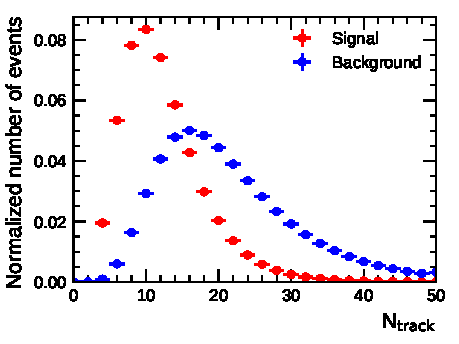
\includegraphics{./figures/rnn/ntrk_3p.pdf}
  \caption{Number of tracks for 3-prong taus}
  \label{fig:total_tracks_3p}
\end{figure}

\begin{figure}[htpb]
  \centering
  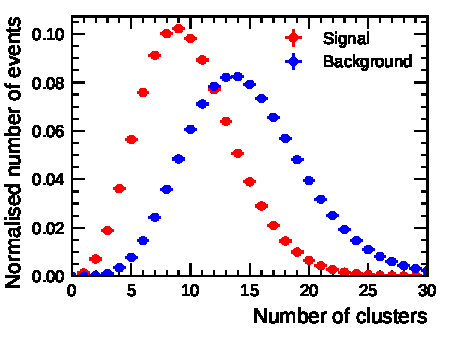
\includegraphics{./figures/rnn/ncls_3p.pdf}
  \caption{Number of clusters for 3-prong taus}
  \label{fig:total_clusters_3p}
\end{figure}

\section{MC Dijet Slices}
Truth $p_\mathrm{T}$ of jet given by anti-$k_\mathrm{T}$ jet algorithm with distance parameter $R=0.6$:
\begin{itemize}
\item[JZ0W] 0 - 20 GeV
\item[JZ1W] 20 - 60 GeV
\item[JZ2W] 60 - 160 GeV
\item[JZ3W] 160 - 400 GeV
\item[JZ4W] 400 - 800 GeV
\item[JZ5W] 800 - 1300 GeV
\item[JZ6W] 1300 - 1800 GeV
\item[JZ7W] 1800 - 2500 GeV
\item[JZ8W] 2500 - 3200 GeV
\end{itemize}

\url{https://svnweb.cern.ch/cern/wsvn/atlasoff/Generators/MC15JobOptions/trunk/share/DSID361xxx/MC15.361021.Pythia8EvtGen_A14NNPDF23LO_jetjet_JZ1W.py}


\url{https://svnweb.cern.ch/cern/wsvn/atlasoff/Generators/MC15JobOptions/trunk/common/Filters/JetFilterAkt6.py}


\url{https://svnweb.cern.ch/cern/wsvn/atlasoff/Generators/MC15JobOptions/trunk/common/Filters/JetFilter_JZX_Fragment.py}

\subsection{Preproduction Taus}

\begin{lstlisting}[basicstyle=\small\ttfamily, breaklines=true]
  mc16_13TeV.425200.Pythia8EvtGen_A14NNPDF23LO_Gammatautau_MassWeight.merge.AOD.e5468_s2997_r9064_r8996
\end{lstlisting}

\subsection{MC16A Taus}
\label{sec:app_mc16a_taus}

\begin{lstlisting}[basicstyle=\small\ttfamily, breaklines=true]
  mc16_13TeV.425200.Pythia8EvtGen_A14NNPDF23LO_Gammatautau_MassWeight.merge.AOD.e5468_s3126_r9364_r9315
\end{lstlisting}

\subsection{Preproduction Dijets}

\begin{lstlisting}[basicstyle=\small\ttfamily, breaklines=true]
  mc16_13TeV.361021.Pythia8EvtGen_A14NNPDF23LO_jetjet_JZ1W.merge.AOD.e3569_s2997_r9064_r8996
  mc16_13TeV.361022.Pythia8EvtGen_A14NNPDF23LO_jetjet_JZ2W.merge.AOD.e3668_s2997_r9064_r9078
  mc16_13TeV.361023.Pythia8EvtGen_A14NNPDF23LO_jetjet_JZ3W.merge.AOD.e3668_s2997_r9064_r8996
  mc16_13TeV.361024.Pythia8EvtGen_A14NNPDF23LO_jetjet_JZ4W.merge.AOD.e3668_s2997_r9064_r9078
  mc16_13TeV.361025.Pythia8EvtGen_A14NNPDF23LO_jetjet_JZ5W.merge.AOD.e3668_s2997_r9064_r8996
  mc16_13TeV.361026.Pythia8EvtGen_A14NNPDF23LO_jetjet_JZ6W.merge.AOD.e3569_s2997_r9064_r9078
\end{lstlisting}

\subsection{Upgrade Samples}
Gammatautau (extended layout \cite{itk_layout_slides}):
\begin{lstlisting}[basicstyle=\small\ttfamily, breaklines=true]
  mc15_14TeV.361247.PowhegPythia8EvtGen_AZNLOCTEQ6L1_Ztautau_new.recon.AOD.e4805_s2987_s2999_r8820
  mc15_14TeV.301040.PowhegPythia8EvtGen_AZNLOCTEQ6L1_DYtautau_120M180.recon.AOD.e5323_s2987_s2999_r8820
  mc15_14TeV.301041.PowhegPythia8EvtGen_AZNLOCTEQ6L1_DYtautau_180M250.recon.AOD.e5323_s2987_s2999_r8820
  mc15_14TeV.301042.PowhegPythia8EvtGen_AZNLOCTEQ6L1_DYtautau_250M400.recon.AOD.e5323_s2987_s2999_r8820
  mc15_14TeV.301043.PowhegPythia8EvtGen_AZNLOCTEQ6L1_DYtautau_400M600.recon.AOD.e5323_s2987_s2999_r8820
  mc15_14TeV.301044.PowhegPythia8EvtGen_AZNLOCTEQ6L1_DYtautau_600M800.recon.AOD.e5323_s2987_s2999_r8820
  mc15_14TeV.301045.PowhegPythia8EvtGen_AZNLOCTEQ6L1_DYtautau_800M1000.recon.AOD.e5323_s2987_s2999_r8820
  mc15_14TeV.301046.PowhegPythia8EvtGen_AZNLOCTEQ6L1_DYtautau_1000M1250.recon.AOD.e5323_s2987_s2999_r8820
  mc15_14TeV.301047.PowhegPythia8EvtGen_AZNLOCTEQ6L1_DYtautau_1250M1500.recon.AOD.e5323_s2987_s2999_r8820
  mc15_14TeV.301048.PowhegPythia8EvtGen_AZNLOCTEQ6L1_DYtautau_1500M1750.recon.AOD.e5323_s2987_s2999_r8820
  mc15_14TeV.301049.PowhegPythia8EvtGen_AZNLOCTEQ6L1_DYtautau_1750M2000.recon.AOD.e5323_s2987_s2999_r8820
  mc15_14TeV.301050.PowhegPythia8EvtGen_AZNLOCTEQ6L1_DYtautau_2000M2250.recon.AOD.e5323_s2987_s2999_r8820
  mc15_14TeV.301051.PowhegPythia8EvtGen_AZNLOCTEQ6L1_DYtautau_2250M2500.recon.AOD.e5323_s2987_s2999_r8820
  mc15_14TeV.301052.PowhegPythia8EvtGen_AZNLOCTEQ6L1_DYtautau_2500M2750.recon.AOD.e5323_s2987_s2999_r8820
  mc15_14TeV.301053.PowhegPythia8EvtGen_AZNLOCTEQ6L1_DYtautau_2750M3000.recon.AOD.e5323_s2987_s2999_r8820
  mc15_14TeV.301054.PowhegPythia8EvtGen_AZNLOCTEQ6L1_DYtautau_3000M3500.recon.AOD.e5323_s2987_s2999_r8820
  mc15_14TeV.301055.PowhegPythia8EvtGen_AZNLOCTEQ6L1_DYtautau_3500M4000.recon.AOD.e5323_s2987_s2999_r8820
  mc15_14TeV.301056.PowhegPythia8EvtGen_AZNLOCTEQ6L1_DYtautau_4000M4500.recon.AOD.e5323_s2987_s2999_r8820
  mc15_14TeV.301057.PowhegPythia8EvtGen_AZNLOCTEQ6L1_DYtautau_4500M5000.recon.AOD.e5323_s2987_s2999_r8820
  mc15_14TeV.301058.PowhegPythia8EvtGen_AZNLOCTEQ6L1_DYtautau_5000M.recon.AOD.e5323_s2987_s2999_r8820
\end{lstlisting}
Dijets (extended layout):
\begin{lstlisting}[basicstyle=\small\ttfamily, breaklines=true]
  mc15_14TeV.147910.Pythia8_AU2CT10_jetjet_JZ0W.recon.AOD.e2403_s2987_s2999_r8820
  mc15_14TeV.147911.Pythia8_AU2CT10_jetjet_JZ1W.recon.AOD.e2403_s2987_s2999_r8820
  mc15_14TeV.147912.Pythia8_AU2CT10_jetjet_JZ2W.recon.AOD.e2403_s2987_s2999_r8820
  mc15_14TeV.147913.Pythia8_AU2CT10_jetjet_JZ3W.recon.AOD.e2403_s2987_s2999_r8820
  mc15_14TeV.147914.Pythia8_AU2CT10_jetjet_JZ4W.recon.AOD.e2403_s2987_s2999_r8820
  mc15_14TeV.147915.Pythia8_AU2CT10_jetjet_JZ5W.recon.AOD.e2403_s2987_s2999_r8820
  mc15_14TeV.147916.Pythia8_AU2CT10_jetjet_JZ6W.recon.AOD.e2403_s2987_s2999_r8820
  mc15_14TeV.147917.Pythia8_AU2CT10_jetjet_JZ7W.recon.AOD.e2403_s2987_s2999_r8820
\end{lstlisting}


\clearpage
\section{Tau-ID Variables}

\subsection{1-prong}
\begin{figure}[!ht]
  \begin{subfigure}{0.5\textwidth}
    \centering
    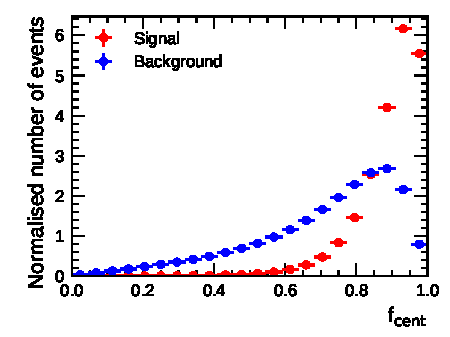
\includegraphics{./figures/baseline_bdt_vars/1p/centFrac.pdf}
  \end{subfigure}%
  \begin{subfigure}{0.5\textwidth}
    \centering
    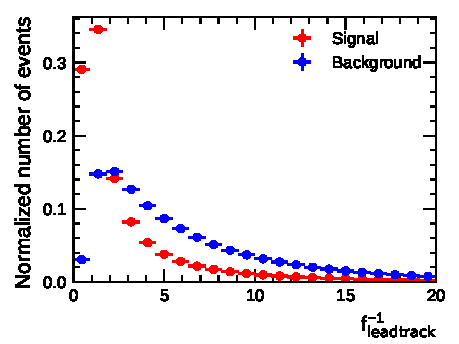
\includegraphics{./figures/baseline_bdt_vars/1p/etOverPtLeadTrk.pdf}
  \end{subfigure}
  \begin{subfigure}{0.5\textwidth}
    \centering
    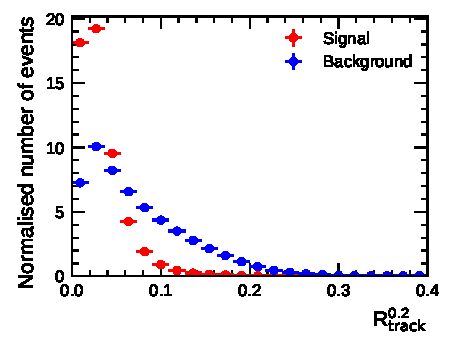
\includegraphics{./figures/baseline_bdt_vars/1p/innerTrkAvgDist.pdf}
  \end{subfigure}%
  \begin{subfigure}{0.5\textwidth}
    \centering
    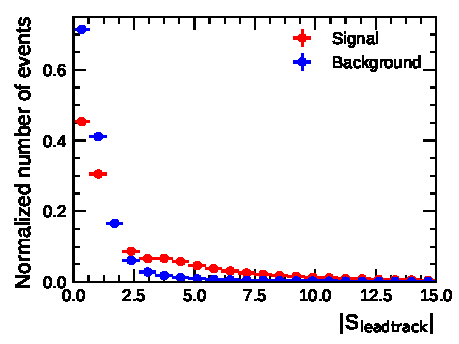
\includegraphics{./figures/baseline_bdt_vars/1p/absipSigLeadTrk.pdf}
  \end{subfigure}
  \begin{subfigure}{0.5\textwidth}
    \centering
    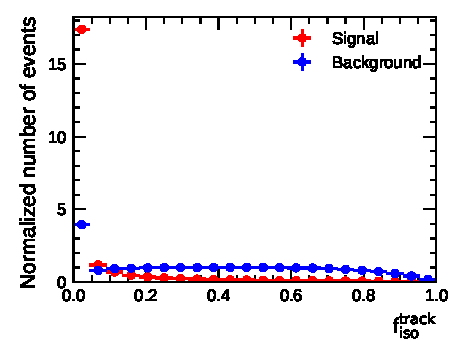
\includegraphics{./figures/baseline_bdt_vars/1p/SumPtTrkFrac.pdf}
  \end{subfigure}%
  \begin{subfigure}{0.5\textwidth}
    \centering
    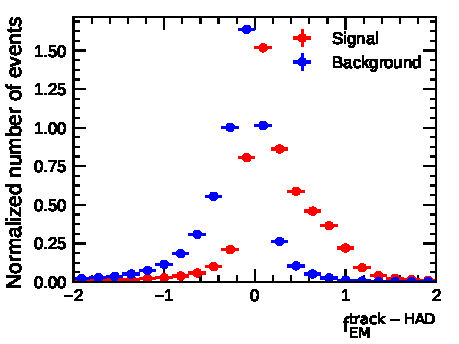
\includegraphics{./figures/baseline_bdt_vars/1p/ChPiEMEOverCaloEME.pdf}
  \end{subfigure}
  \caption{Variables used in Tau-ID BDT. \mytodo{Rename innerTrkAvgDist x-label}}
  \label{fig:bdt_vars_1p_overlays}
\end{figure}

\begin{figure}[!ht]\ContinuedFloat
  \begin{subfigure}{0.5\textwidth}
    \centering
    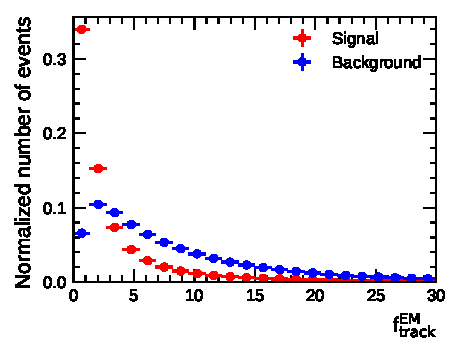
\includegraphics{./figures/baseline_bdt_vars/1p/EMPOverTrkSysP.pdf}
  \end{subfigure}%
  \begin{subfigure}{0.5\textwidth}
    \centering
    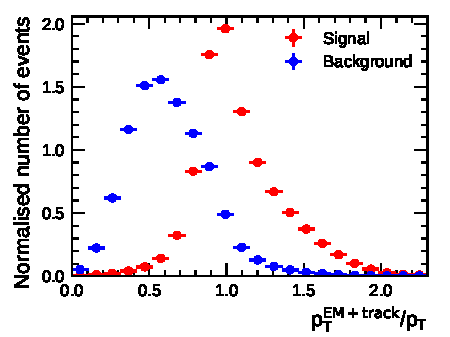
\includegraphics{./figures/baseline_bdt_vars/1p/ptRatioEflowApprox.pdf}
  \end{subfigure}
  \begin{subfigure}{0.5\textwidth}
    \centering
    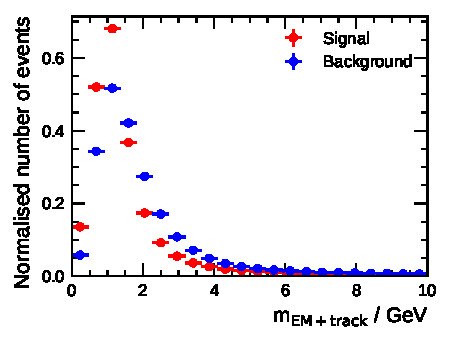
\includegraphics{./figures/baseline_bdt_vars/1p/mEflowApprox.pdf}
  \end{subfigure}
  \caption[]{Variables used in Tau-ID BDT}
\end{figure}

\clearpage
\subsection{3-prong}

\begin{figure}[!ht]
  \begin{subfigure}{0.5\textwidth}
    \centering
    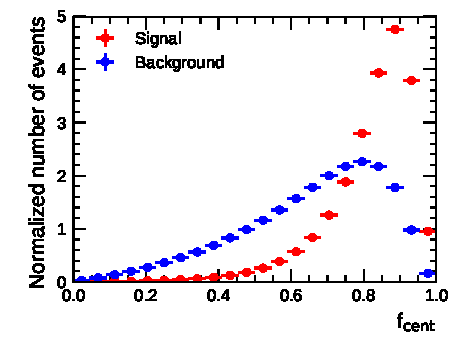
\includegraphics{./figures/baseline_bdt_vars/3p/centFrac.pdf}
  \end{subfigure}%
  \begin{subfigure}{0.5\textwidth}
    \centering
    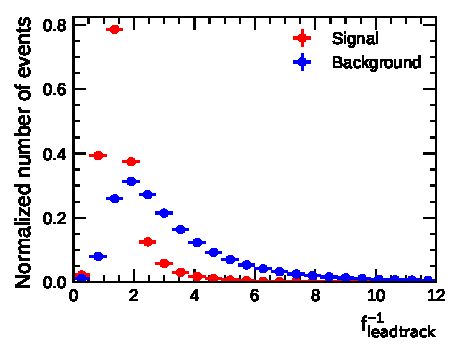
\includegraphics{./figures/baseline_bdt_vars/3p/etOverPtLeadTrk.pdf}
  \end{subfigure}
  \begin{subfigure}{0.5\textwidth}
    \centering
    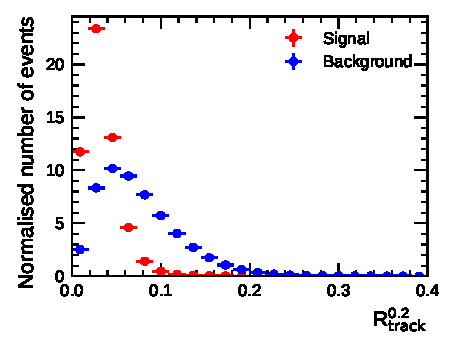
\includegraphics{./figures/baseline_bdt_vars/3p/innerTrkAvgDist.pdf}
  \end{subfigure}%
  \begin{subfigure}{0.5\textwidth}
    \centering
    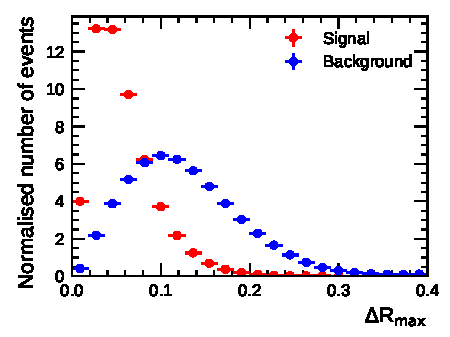
\includegraphics{./figures/baseline_bdt_vars/3p/dRmax.pdf}
  \end{subfigure}
  \begin{subfigure}{0.5\textwidth}
    \centering
    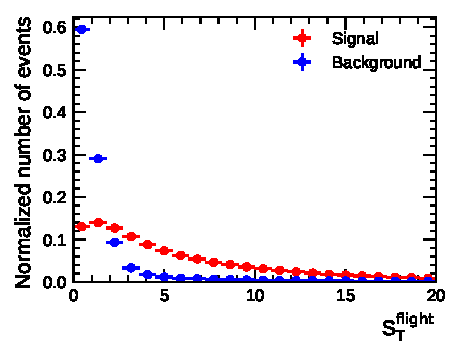
\includegraphics{./figures/baseline_bdt_vars/3p/trFlightPathSig.pdf}
  \end{subfigure}%
  \begin{subfigure}{0.5\textwidth}
    \centering
    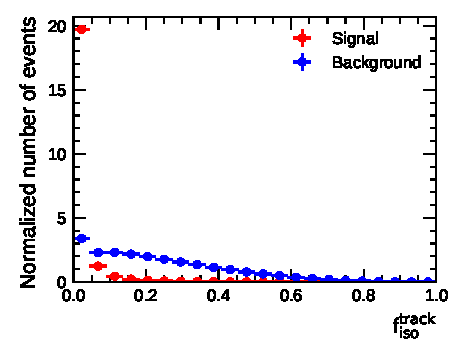
\includegraphics{./figures/baseline_bdt_vars/3p/SumPtTrkFrac.pdf}
  \end{subfigure}%
  \caption{Variables used in Tau-ID BDT\mytodo{rename innerTrkAvgDist x-label}}
  \label{fig:bdt_vars_3p_overlays}
\end{figure}

\begin{figure}[!ht]\ContinuedFloat
  \begin{subfigure}{0.5\textwidth}
    \centering
    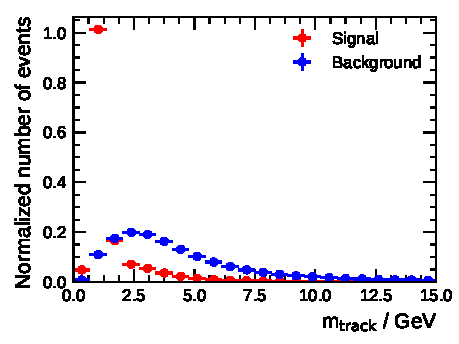
\includegraphics{./figures/baseline_bdt_vars/3p/massTrkSys.pdf}
  \end{subfigure}%
  \begin{subfigure}{0.5\textwidth}
    \centering
    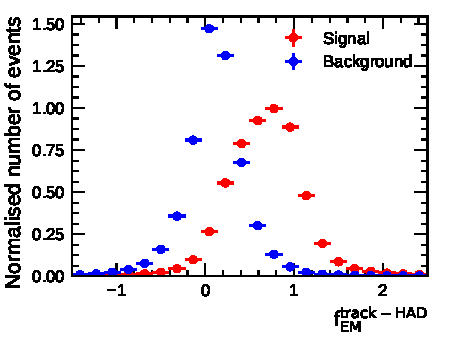
\includegraphics{./figures/baseline_bdt_vars/3p/ChPiEMEOverCaloEME.pdf}
  \end{subfigure}
  \begin{subfigure}{0.5\textwidth}
    \centering
    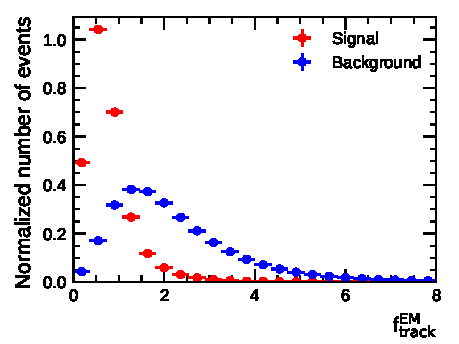
\includegraphics{./figures/baseline_bdt_vars/3p/EMPOverTrkSysP.pdf}
  \end{subfigure}%
  \begin{subfigure}{0.5\textwidth}
    \centering
    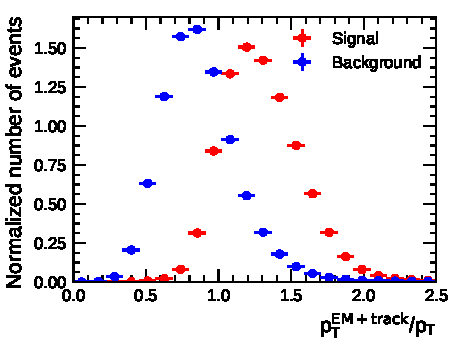
\includegraphics{./figures/baseline_bdt_vars/3p/ptRatioEflowApprox.pdf}
  \end{subfigure}
  \begin{subfigure}{0.5\textwidth}
    \centering
    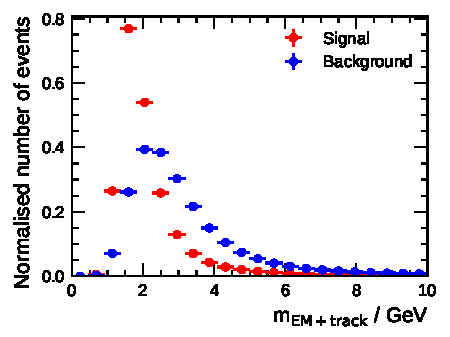
\includegraphics{./figures/baseline_bdt_vars/3p/mEflowApprox.pdf}
  \end{subfigure}
  \caption[]{Variables used in Tau-ID BDT}
\end{figure}

\clearpage
\section{Decay Mode Classification using Recurrent Neural Networks}
\subsection{Baseline Probabilities}

\begin{figure}[!ht]
  \begin{subfigure}{0.48\textwidth}
    \centering
    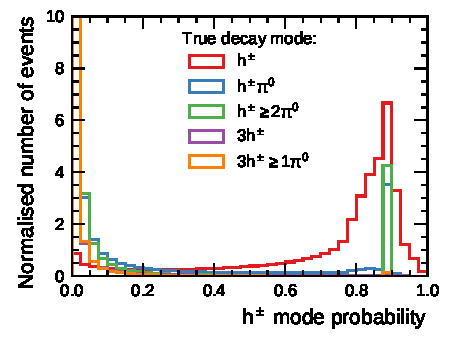
\includegraphics{./figures/decay_mode_classification/mode_proba_baseline_ptcut_1_5/proba_1p0n.pdf}
  \end{subfigure}\hfill
  \begin{subfigure}{0.48\textwidth}
    \centering
    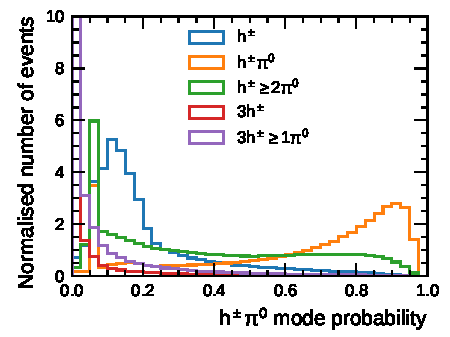
\includegraphics{./figures/decay_mode_classification/mode_proba_baseline_ptcut_1_5/proba_1p1n.pdf}
  \end{subfigure}
  \begin{subfigure}{0.48\textwidth}
    \centering
    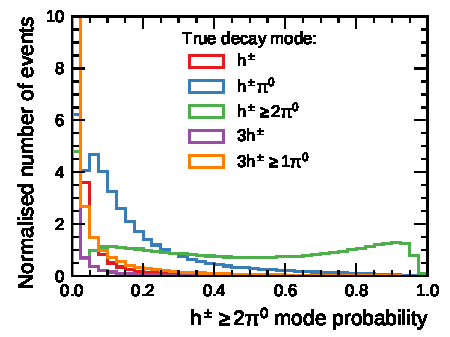
\includegraphics{./figures/decay_mode_classification/mode_proba_baseline_ptcut_1_5/proba_1pXn.pdf}
  \end{subfigure}\hfill
  \begin{subfigure}{0.48\textwidth}
    \centering
    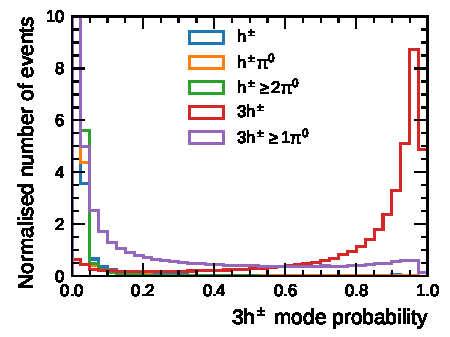
\includegraphics{./figures/decay_mode_classification/mode_proba_baseline_ptcut_1_5/proba_3p0n.pdf}
  \end{subfigure}
  \begin{subfigure}{0.48\textwidth}
    \centering
    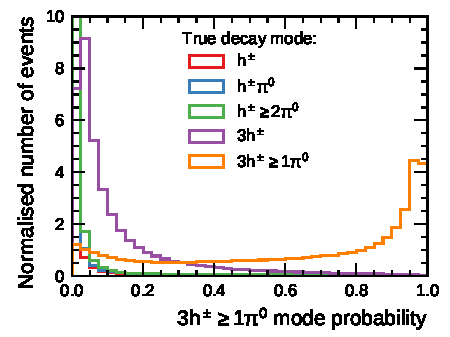
\includegraphics{./figures/decay_mode_classification/mode_proba_baseline_ptcut_1_5/proba_3pXn.pdf}
  \end{subfigure}%

  \caption{Multi-class probabilities for the Baseline RNN}
  \label{fig:rnn_multiclass_proba_baseline}
\end{figure}

\clearpage
\subsection{Combined Probabilities}

\begin{figure}[!ht]
  \begin{subfigure}{0.48\textwidth}
    \centering
    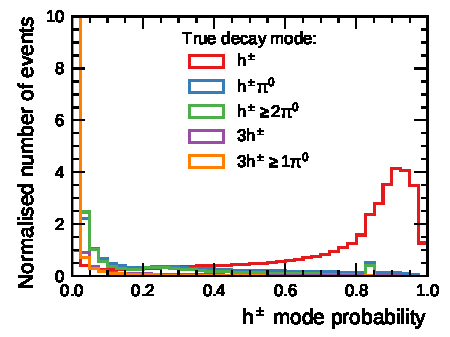
\includegraphics{./figures/decay_mode_classification/combined_proba/proba_1p0n.pdf}
  \end{subfigure}\hfill
  \begin{subfigure}{0.48\textwidth}
    \centering
    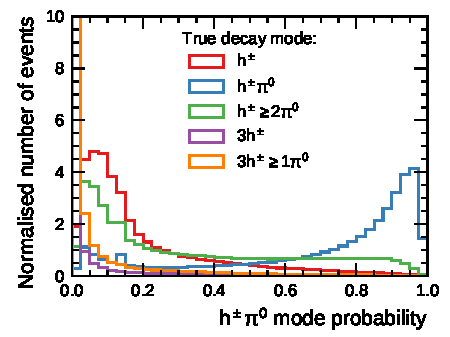
\includegraphics{./figures/decay_mode_classification/combined_proba/proba_1p1n.pdf}
  \end{subfigure}
  \begin{subfigure}{0.48\textwidth}
    \centering
    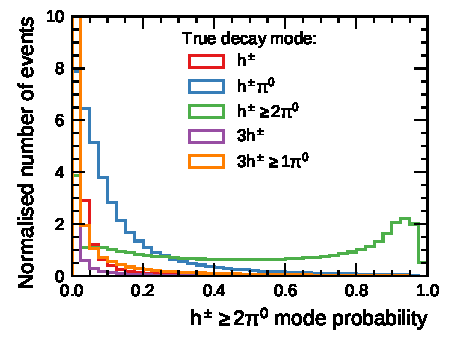
\includegraphics{./figures/decay_mode_classification/combined_proba/proba_1pXn.pdf}
  \end{subfigure}\hfill
  \begin{subfigure}{0.48\textwidth}
    \centering
    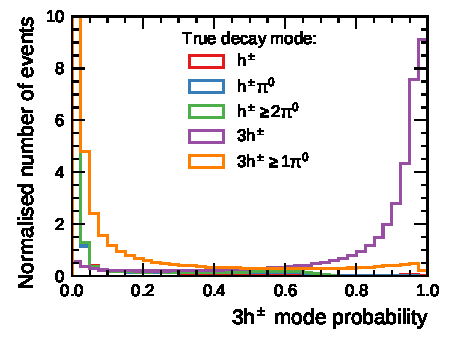
\includegraphics{./figures/decay_mode_classification/combined_proba/proba_3p0n.pdf}
  \end{subfigure}
  \begin{subfigure}{0.48\textwidth}
    \centering
    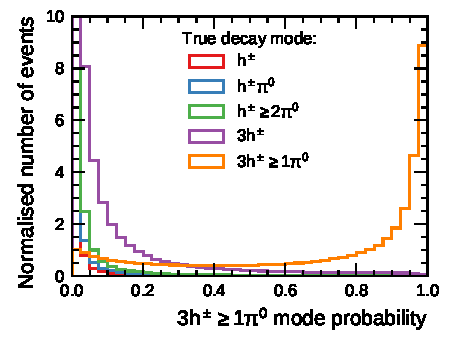
\includegraphics{./figures/decay_mode_classification/combined_proba/proba_3pXn.pdf}
  \end{subfigure}%

  \caption{Multi-class probabilities for the Combined RNN}
  \label{fig:rnn_multiclass_proba_combined}
\end{figure}

\clearpage
\section{BDT: Recursive Feature Elimination}

\begin{figure}[htb]
  \centering
  \begin{subfigure}[t]{0.33\textwidth}
    \centering
    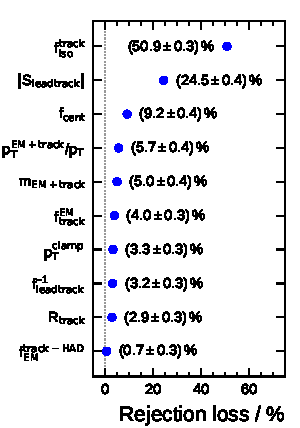
\includegraphics{./figures/bdt_perf/var_importance/1p_iter1.pdf}
    \subcaption{Iteration 1}
  \end{subfigure}
  \begin{subfigure}[t]{0.33\textwidth}
    \centering
    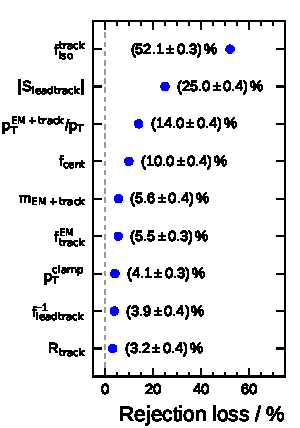
\includegraphics{./figures/bdt_perf/var_importance/1p_iter2.pdf}
    \subcaption{Iteration 2}
  \end{subfigure}
  \caption{Variable importance (1-prong). Averaged rejection loss over a
    gamma-tautau like dijet spectrum. Tight working point.}
  \label{fig:variable_importance_1p_app}
\end{figure}

\begin{figure}[htb]
  \centering
  \begin{subfigure}[t]{0.32\textwidth}
    \centering
    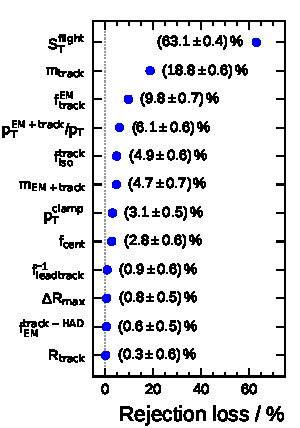
\includegraphics{./figures/bdt_perf/var_importance/3p_iter1.pdf}
    \subcaption{Iteration 1}
  \end{subfigure}
  \begin{subfigure}[t]{0.32\textwidth}
    \centering
    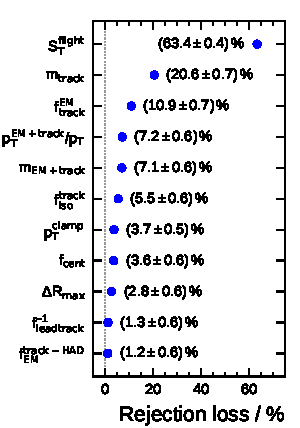
\includegraphics{./figures/bdt_perf/var_importance/3p_iter2.pdf}
    \subcaption{Iteration 2}
  \end{subfigure}
  \begin{subfigure}[t]{0.32\textwidth}
    \centering
    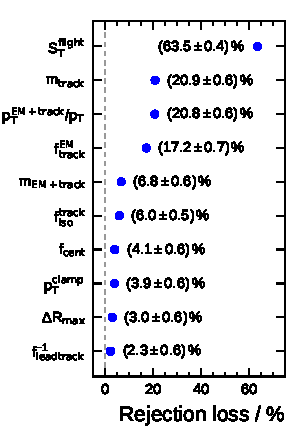
\includegraphics{./figures/bdt_perf/var_importance/3p_iter3.pdf}
    \subcaption{Iteration 3}
  \end{subfigure}

  \caption{Variable importance (3-prong). Averaged rejection loss over a
    gamma-tautau like dijet spectrum. Tight working point.}
  \label{fig:variable_importance_3p_app}
\end{figure}

\clearpage
\section{Post-Optimisation Working Points}

\begin{figure}[htb]
  \centering
  \begin{subfigure}{0.48\textwidth}
    \centering
    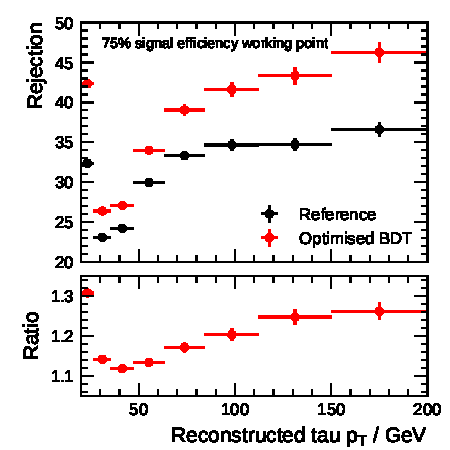
\includegraphics{./figures/bdt_perf/post_optimisation/rejection_medium_1p.pdf}
  \end{subfigure}\hfill
  \begin{subfigure}{0.48\textwidth}
    \centering
    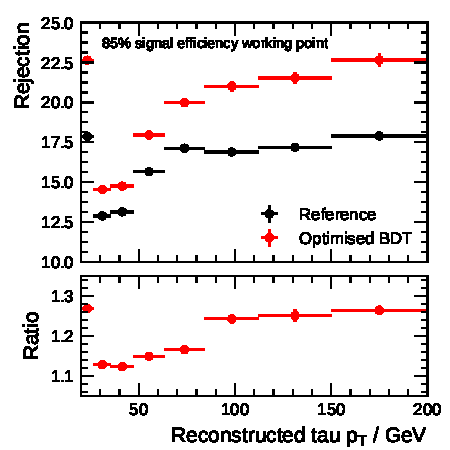
\includegraphics{./figures/bdt_perf/post_optimisation/rejection_loose_1p.pdf}
  \end{subfigure}
  \caption{1-prong}
\end{figure}

\begin{figure}[htb]
  \centering
  \begin{subfigure}{0.48\textwidth}
    \centering
    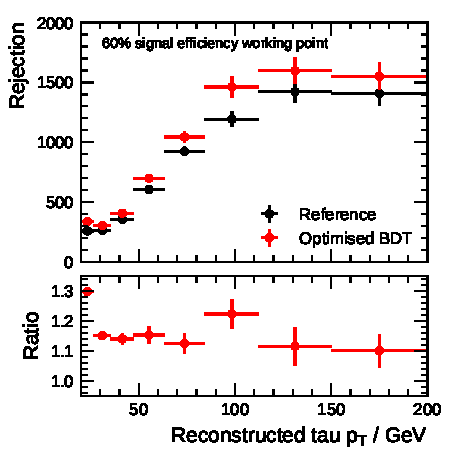
\includegraphics{./figures/bdt_perf/post_optimisation/rejection_medium_3p.pdf}
  \end{subfigure}\hfill
  \begin{subfigure}{0.48\textwidth}
    \centering
    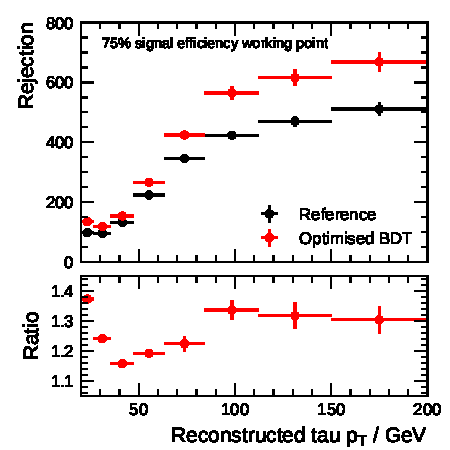
\includegraphics{./figures/bdt_perf/post_optimisation/rejection_loose_3p.pdf}
  \end{subfigure}
  \caption{3-prong}
\end{figure}

\clearpage
\section{Rejection vs.\ Initiating Parton}
\begin{figure}[htb]
  \centering
  \begin{subfigure}[t]{0.48\textwidth}
    \centering
    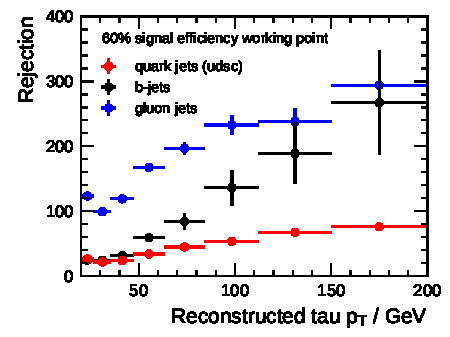
\includegraphics{./figures/bdt_perf/parton/truth_parton_1p.pdf}
    \caption{1-prong}
  \end{subfigure}\hfill
  \begin{subfigure}[t]{0.48\textwidth}
    \centering
    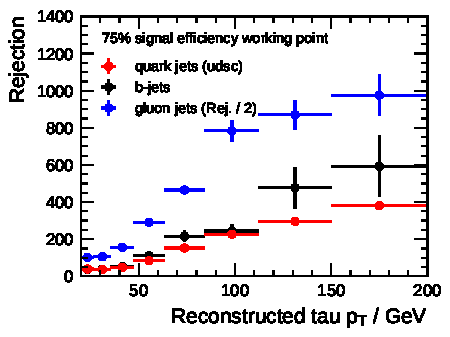
\includegraphics{./figures/bdt_perf/parton/truth_parton_3p.pdf}
    \caption{3-prong. Loose working point (Tight has too much rejection for
      limited stats)}
  \end{subfigure}
  \caption{Rejection vs initiating parton}
\end{figure}

\clearpage
\section{Decay Mode Classification Experiments}
\label{sec:app_decay_mode_exp}
\begin{figure}[htb]
  \begin{subfigure}[t]{0.48\textwidth}
    \centering
    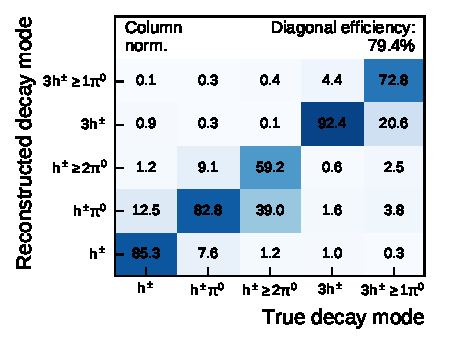
\includegraphics{./figures/decay_mode_classification/experiments/mig_mat_conversions.pdf}
    \subcaption{Migration matrix}
  \end{subfigure}\hfill
  \begin{subfigure}[t]{0.48\textwidth}
    \centering
    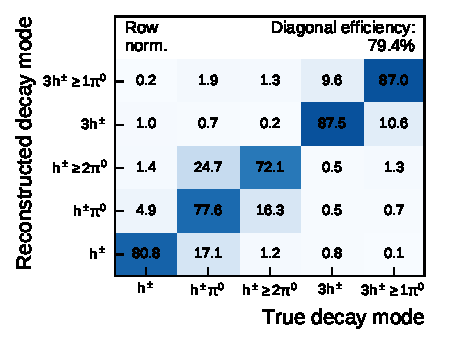
\includegraphics{./figures/decay_mode_classification/experiments/comp_mat_conversions.pdf}
    \subcaption{Composition matrix}
  \end{subfigure}
  \caption{Conversion tracks}
\end{figure}

\begin{figure}[htb]
  \begin{subfigure}[t]{0.48\textwidth}
    \centering
    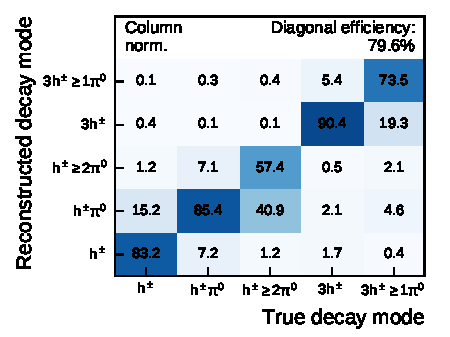
\includegraphics{./figures/decay_mode_classification/experiments/mig_mat_shots.pdf}
    \subcaption{Migration matrix}
  \end{subfigure}\hfill
  \begin{subfigure}[t]{0.48\textwidth}
    \centering
    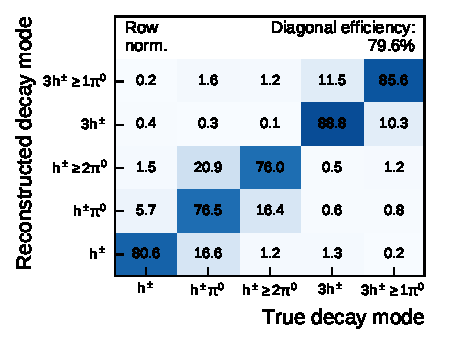
\includegraphics{./figures/decay_mode_classification/experiments/comp_mat_shots.pdf}
    \subcaption{Composition matrix}
  \end{subfigure}
  \caption{Shots}
\end{figure}

\begin{figure}[htb]
  \begin{subfigure}[t]{0.48\textwidth}
    \centering
    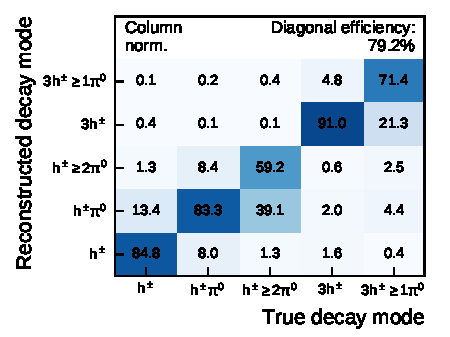
\includegraphics{./figures/decay_mode_classification/experiments/mig_mat_moments.pdf}
    \subcaption{Migration matrix}
  \end{subfigure}\hfill
  \begin{subfigure}[t]{0.48\textwidth}
    \centering
    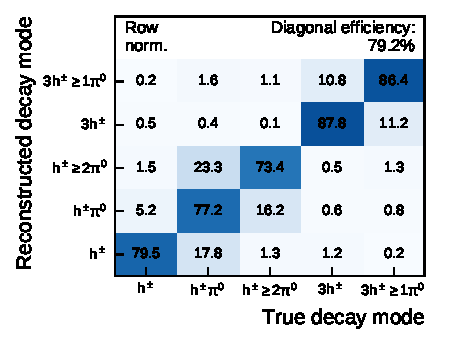
\includegraphics{./figures/decay_mode_classification/experiments/comp_mat_moments.pdf}
    \subcaption{Composition matrix}
  \end{subfigure}
  \caption{Add.\ cluster moments}
\end{figure}

\begin{figure}[htb]
  \begin{subfigure}[t]{0.48\textwidth}
    \centering
    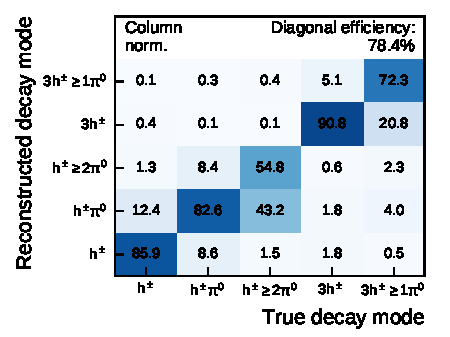
\includegraphics{./figures/decay_mode_classification/experiments/mig_mat_hadronic_pfos.pdf}
    \subcaption{Migration matrix}
  \end{subfigure}\hfill
  \begin{subfigure}[t]{0.48\textwidth}
    \centering
    \includegraphics{./figures/decay_mode_classification/experiments/comp_mat_hadronic_pfos.pdf}
    \subcaption{Composition matrix}
  \end{subfigure}
  \caption{Hadronic PFOs}
\end{figure}

\begin{figure}[htb]
  \begin{subfigure}[t]{0.48\textwidth}
    \centering
    \includegraphics{./figures/decay_mode_classification/experiments/mig_mat_sub_e_2.pdf}
    \subcaption{Migration matrix}
  \end{subfigure}\hfill
  \begin{subfigure}[t]{0.48\textwidth}
    \centering
    \includegraphics{./figures/decay_mode_classification/experiments/comp_mat_sub_e_2.pdf}
    \subcaption{Composition matrix}
  \end{subfigure}
  \caption{$p_\text{T}$-fraction}
\end{figure}


\clearpage
\section{TODOS}
\listoftodos

%%% Local Variables:
%%% mode: latex
%%% TeX-master: "mythesis"
%%% End:
